\section{Digital signalbehandling (DSP)}
\label{DSP}
\index{digital signalbehandling}
\index{digital signal processing (DSP)}
\index{DSP|see {digital signalbehandling}}
\index{Software Defined Radio}
\index{SDR|see {Software Defined Radio}}
\index{FPGA}

\emph{Digital signalbehandling} (eng. \emph{Digital Signal Processing (DSP)})
har blivit allt viktigare i vardagen och så även inom amatörradion i och med
att \emph{Software Defined Radio (SDR)} blivit en viktig del i allt fler
radior, liksom användning av vanliga datorer.

I grunden bygger den på att man digitaliserar signalerna, behandlar dem
digitalt i exempelvis en processor eller programmerbar logik (FPGA) och sedan
omvandlar dem till analoga signaler igen.

Om man har en särskilt processor för att göra det kallar man den för en
\emph{Digital Signalprocessor (DSP)}.
Behandlingen kan även göras av dedikerad logik, alltså logik avsedd för speciellt
ändamål, som inte kan programmeras på normalt sätt som en processor. Det är fortfarande
\emph{Digital Signalbehandling}, men den används nu mer mest för de delar av
signlbehandlingen där man behöver utföra samma standardiserade jobb fort och
effektivt.
En processor kan i stället utföra de mindre frekventa jobben som därmed kan
tillåtas vara mer komplexa.

En GPS-mottagare är ett exempel på en sådan mottagare där dedikerad hårdvara
hanterar många miljoner sampel per sekund, men som reducerar dem till några värden
per millisekund som sedan behandlas vidare i en processor.

För att kunna förstå detta behöver vi gå igenom grunderna i konvertering av
signalerna från analogt till digitalt och tillbaka från digitalt till analogt.

\subsection{Sampling och kvantisering}
\harec{a}{1.10.1}{1.10.1}
\index{sampling}
\index{samplingstakt}
\index{sample rate}
\index{samplingsperiod}
\index{sample (S)}
\index{enheter!sample (S)}
\index{tidsdiskret}
\index{kvantisering}
\index{quantize}
\index{Pulse Code Modulation (PCM)}
\index{PCM}

Analoga signaler är vad vi kallar för kontinuerliga i tid. Hos dessa varierar spänning och
ström kontinuerligt så snabbt att vi kan hantera det fulla radiospektrumet och mer därtill.
Detta fungerar dock inte så väl i den digitala världen.
Där vill vi dels ha värden i digital form, så vi behöver omvandla våra spänningar
och strömmar till tal, och dels behöver vi göra det i en jämn takt.

\emph{Sampling} är ett engelskt ord som betyder att ta strickprov eller att göra ett urval.
Vi tar ett stickprov (sampel) då och då, och i detta sammanhang gör vi det i en jämn takt,
\emph{samplingstakten} (eng. \emph{sample rate}).
Denna benämner vi ofta med \(f_S\) och begreppet \emph{samplingsperiodtid}
\(T_S=\frac{1}{f_S}\) används också.
Samplingstakten är alltså den jämna takt varmed vi får värden.
Ibland säger man lite slarvigt att samplingstakten är exempelvis 1~MHz, men det
mer korrekta är att den är 1~MS/s, det vill säga 1 miljon sampel per sekund.

Bild \ref{fig:BildII1-37} illustrerar hur en analog signal samplas och
kvantiseras i en ADC, för att behandlas i en DSP, för att därefter konverteras
till analog signal med DAC och filtreras.

\mediumfig[0.9]{images/cropped_pdfs/bild_2_1-37.pdf}{Sampling med ADC, DSP och DAC för att återvinna analog signal}{fig:BildII1-37}

Medan sampling är den process som ger oss \emph{tidsdiskreta} värden istället
för tidskontinuerliga värden så är värdena fortfarande inte representerade som
tal, det vill säga värdesdiskreta istället för värdeskontinuerliga.
För att åstadkomma detta behöver man omvandla värdena till fasta nivåer, en
process som kallas för \emph{kvantisering} (eng. \emph{quantize}).

Vid kvantisering har man ofta ett fixt avstånd mellan stegen på en
trappstege av värden. Varje steg kallas ibland för kvantiseringssteg och
storleken på varje kvantiseringssteg avgör därmed hur hög upplösning man får.
Har man till exempel ett kvantiseringssteg på 0,1~V så blir 0 till 0,1~V tolkat som
0, 0,1--0,2~V blir tolkat som 1 och så vidare.
Bild \ref{fig:BildII1-37} visar hur kvantiseringen sker i ADC-steget.

Denna sista del i att omvandla de kvantiserade talen till värden kallas
\emph{Pulse Code Modulation (PCM)}.
Omvandlingen kan även ske olinjärt, alltså med olika avstånd mellan stegen i
kvantiseringstrappan, vilket nyttjats för datakompression i telefonisystem.

\subsection{Minsta samplingsfrekvensen}
\harec{a}{1.10.2}{1.10.2}
\index{nyquistfrekvens}
\index{Nyquist-Shannons samplingsteorem}

\begin{quote}
\emph{Denna frekvens kallas för nyquistfrekvensen efter Harry Nyquist (1889--1976),
från Stora Kil i Värmland, efter hans banbrytande arbete på Bell laboratories
som han publicerade åren 1924 och 1928. Den ingår i \emph{Nyquist-Shannons
samplingsteorem} (eng. \emph{Nyquist-Shannon sampling theorem}).}
\end{quote}

Vår nya begreppsvärld har några inneboende begränsningar, en av dem är minsta
samplingsfrekvensen.
Den lägsta frekvensen vi kan hantera i vårt samplade material är fasta värden
(eller DC som man oftast säger) medan den högsta är den när man alternerar
mellan två värden, säg -1 +1 -1 +1 vilket ju ger hälften av samplingstakten
\(f_S\), för perioden för sekvensen blir \(T = 2T_S\) och därmed
\(f=\frac{1}{T}=\frac{1}{2T_S}=\frac{f_S}{2}\).

\subsection{Faltning}
\harec{a}{1.10.3}{1.10.3}
\index{faltning}
\index{convolution}
\index{konvolution}
\index{linjärt tidsinvariant filter}
\index{linear time-invariant filter}
\index{LTI}

Filtrering i den digitala domänen, eller egentligen den tidsdiskreta domänen,
kan beskrivas som att filtrets impulsrespons appliceras på signalen. Denna
process kallas för \emph{faltning} (ty. \emph{faltung} ''vikning'') eller ibland
\emph{konvolution} (eng. \emph{convolution}).
Man kan se det som att varje enskilt sampel kommer att spela upp hela filtrets
svängning med sin amplitud, och responsen från alla sampel blir därför summan
av alla dessa.

Den matematiskt sinnade kan då använda formeln

\(y(n) = \sum_{m=0}^{N-1} x(n-m)h(m)\)

där \(x(n)\) är den inkommande sampelströmmen och \(n\) är indexet för det
n:te samplet, \(h(m)\) är filtrets respons och slutligen \(y(n)\) är de utgående
samplen.
Denna summering är densamma som beskrivits ovan och skildrar processen
i tidsplanet, det vill säga när vi uttrycker amplituden som funktion av tid.

Motsvarande process kan även utföras i frekvensplanet, det vill säga när vi 
istället uttrycker amplituden som funktion av frekvens.
Om vi då även har konverterat filtrets egenskaper, gör vi helt enkelt en
multiplikation av signal och filter för varje frekvens:

\(Y(f) = X(f)H(f)\)

Bägge representerar faltning, och är viktiga för förståelsen av \emph{linjära
tidsinvarianta} filter (eng. \emph{linear time-invariant (LTI)}) filter,
som är det vi i allmänhet fokuserar på.

\subsection{Antivikningsfilter}
\harec{a}{1.10.4}{1.10.4}
\index{vikning}
\index{aliasing}
\index{antivikningsfilter}
\index{anti-aliasing filter}

Medan bandbredden vi kan representera är begränsad av nyquistfrekvensen så
är däremot inte frekvensen det.
Själva samplingen ger upphov till \emph{vikning} (eng. \emph{aliasing}),
sådan att spektrumet efter halva samplingsfrekvensen blir vänt så att högre
frekvenser blir lägre.
Denna vikning vänder sedan igen när frekvensen blir den hos
samplingsfrekvensen, och spektrumet upprepar sig.
Detta fenomen uppstår alltid när man går mellan kontinuerlig och diskret tid.

\begin{figure*}
\begin{center}
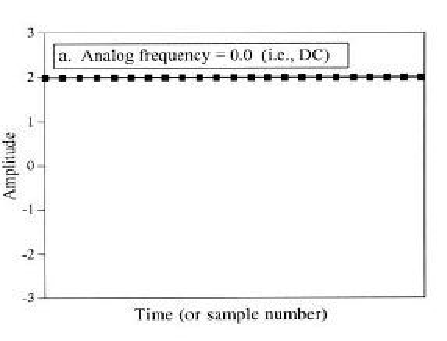
\includegraphics[width=0.45\textwidth]{images/cropped_pdfs/bild_2_1-38.pdf}
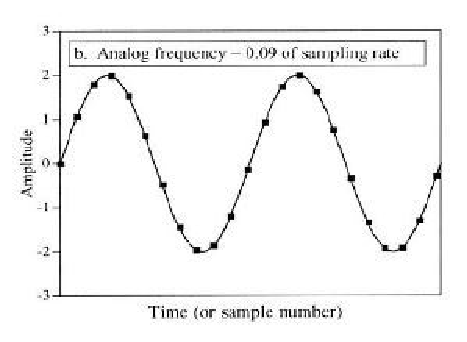
\includegraphics[width=0.45\textwidth]{images/cropped_pdfs/bild_2_1-39.pdf}
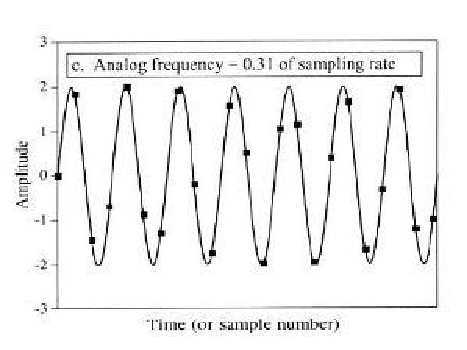
\includegraphics[width=0.45\textwidth]{images/cropped_pdfs/bild_2_1-40.pdf}
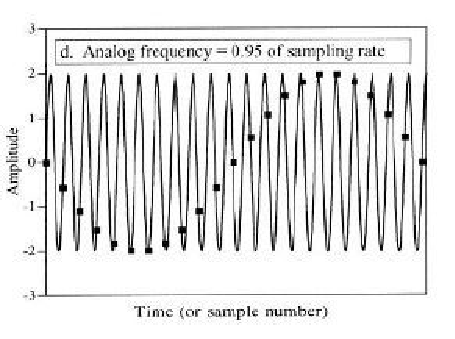
\includegraphics[width=0.45\textwidth]{images/cropped_pdfs/bild_2_1-41.pdf}
\caption{Sampling av DC, 3,6~kHz, 12,4~kHz och 38~kHz med 40~kS/s samplingstakt}
\label{fig:BildII1-38}
\end{center}
\end{figure*}

Bild \ref{fig:BildII1-38} visar hur fyra olika signaler, DC, sinus med
3,6~kHz, 12,4~kHz och 38~kHz, samplas med samplingstakten 40 kS/s.
Fallet med DC är uppenbart enkelt, alla punkterna hamnar på samma spänning.
Vid en lågfrekvent sinus, som fallet är med 3,6~kHz här, får man punkter spridda
över kurvan och de påminner om den ursprungliga sinusen, än mer om man knyter
samman punkterna, vilket antivikningsfiltret i praktiken gör.
En frekvens som är nära nyquistfrekvensen, såsom 12,4~kHz in i 40~kS/s och
dess 20~kHz nyquistfrekvens, så är samplingspunkterna nästa helt alternerande
mellan högsta och lägsta läge. I detta fall är det svårt att se den bakomliggande
sinussignalen för ett otränat öga, men den kan fortfarande rekonstrueras med ett
antialiasingfiltret.
Ett ännu svårare fall är 38~kHz, där punkterna visar en sinus med 2~kHz, då
frekvensen vikt sig ned runt nyquistfrekvensen, och eftersom infrekvensen är
18~kHz över nyquistfrekvensen hamnar den därför 18~kHz under nyquistfrekvensen,
det vill säga på 2~kHz i det här fallet. Denna vikning är det man försöker undvika med
antivikningsfiltret, eftersom toner kan vika sig ned och bli störningar.
Denna vikning sker både vid själva samplingen och även omvänt när man lägger ut
en signal analogt igen. Därför krävs filtrering i bägge riktningarna.

Vid sampling kan alltså högre frekvenser vika ned sig i spektrumet.
Detta är oftast oönskat, varvid man har ett filter före ingången som
undertrycker oönskade signaler.
För exempelvis talsignaler använder man ett lågpassfilter för att undertrycka de
oönskade signalerna högre upp.
Detta filter kan istället användas för ett visst frekvensband för att
konvertera ned detta band i processen, något som är väldigt populärt i
SDR-sammanhang.
I bägge dessa fall är filtret ett \emph{antivikningsfilter} (eng.
\emph{anti-aliasing filter}).

Omvänt, när man ska konvertera från tidsdiskret till tidskontinuerlig
signal så viker sig signalen uppåt i frekvens, och för att undertrycka dessa
oönskade frekvenser används på samma sätt ett antivikningsfilter.
På samma sätt som förut kan man antingen få de låga frekvenserna som för tal
med ett lågpassfilter eller högre upp i ett band med ett lämpligt
bandpassfilter.

Antivikningsfilter kan många gånger vara relativt branta, för de måste
undertrycka andra delar av spektrumet så att dessa inte blir en störning.

Vid varje fall när man använder en annan frekvens än den lägsta upp till
nyquistfrekvensen får man vara omsorgsfull för att se till att man inte viker
det tänkta bandet.
Ofta kombinerar man därför med en separat mixer för att flytta bandet på ett
behändigt sätt, men det förekommer också att man väljer samplingstakten för att
inte vika bandet.

\subsection{ADC/DAC}
\harec{a}{1.10.5}{1.10.5}
\index{ADC}
\index{DAC}

För att hantera dessa delar använder man analog-till-digital-omvandlare
(eng. \emph{Analog-Digital Conversion (ADC)}) samt digital-till-analog-omvandlare 
(eng. \emph{Digital-Analog Conversion (DAC)}).
En ADC tar hand om sampling, kvantisering och PCM-kodning medan en DAC
omvandlar PCM-koden till analog spänning.
Ofta behöver man komplettera med analoga filter, men moderna sigma-delta-omvandlare 
har kraftigt reducerat kraven.

ADC och DAC köper man idag som färdiga integrerade kretsar, inte sällan med
flera kanaler och det finns även de som har bägge integrerade i samma krets.
Utvecklingen har gjort att man idag kan köpa 24-bitars 48~kS/s ADC och DAC med
dynamiskt område bättre än 100~dB för väldigt låg kostnad.
